\documentclass[physics_notes.tex]{subfiles}
\begin{document}
\section{Aula 06 - 13/04/2023}
\subsection{Motivações}
\begin{itemize}
	\item Revisar movimento relativo;
\end{itemize}

\subsection{Movimento Relativo}
Fixada uma origem O, a soma dos vetores representando os corpos A e B
$$
	\vec{r}_{AO} + \vec{r}_{BA} = \vec{r}_{BO}
$$
nos fornece a direção relativa do corpo B com relação a A. Se A e B estão se movendo, ou seja, os vetores deles
possuem dependência no tmepo ($\vec{r}_{AO} = \vec{r}_{AO}(t), \vec{r}_{BO} = \vec{r}_{BO}(t)$), então
$$
	\vec{r}_{BA}(t) = \vec{r}_{BO}(t) + \vec{r}_{AO}(t),
$$
ou seja, a posição relativa de B com relação a A também dependerá do tempo. Além de posição relativa,
podemos definir outros conceitos, tais como a velocidade relativa:
$$
	\vec{v}_{BA}(t) = \frac{d \vec{r}_{BA}(t)}{dt} = \frac{d \vec{r}_{BO}}{dt} + \frac{d \vec{r}_{AO}}{dt} \Rightarrow \vec{v}_{BA}(t) = \vec{v}_{BO}(t)  + \vec{v}_{AO}(t)
$$
e aceleração relativa de modo análogo, i.e., $\vec{a}_{BA}(t) = \vec{a}_{BO}(t) + \vec{a}_{AO}(t).$ Vejamos alguns exemplos
\begin{example}
	Considere um sistema em que um carrinho viaja com velocidade $\vec{v}_{r}$ e tem um passageiro $\vec{v}_{p}$ com ele.
	Ambos se movem para a direita.
	Neste caso, há o sistema referencial de inérca da pessoa dentro do trem. Buscamos descobrir a velocidade da pessoa com relação ao trem.
	De fato, segue que
	$$
		\vec{v}_{p} = \vec{v}_{PT} + \vec{v}_{T}.
	$$
\end{example}
\begin{example}
	Considere um sistema análogo ao anterior, mas, embaixo, há uma plataforma se movendo para a esquerda com velocidade igual à do trem.
	Neste caso, há o sistema referencial de inérca da pessoa dentro do trem. Buscamos descobrir a velocidade da pessoa com relação
	à plataforma. Obtemos
	$$
		\vec{v}_{PT} = \vec{v}_{PT}^{x}\hat{i} + \vec{v}_{PT}^{y}\hat{j}. \Rightarrow \vec{v}_{p} = (\vec{v}_{PT}^{x} + \vec{v}_{T})\hat{i} + \vec{v}_{P}^{y}\hat{j}
	$$
\end{example}
\begin{example}
	(Exemplo 32 do Tipler): Considere um sistema de avião e vento, no qual o módulo da velocidade do avião é de 200km/h e,
	o da velocidade do vento, é 90km/h. O vento é dado por um vetor apontando para a direito, enquanto o avião é um vetor apontando para cima.
	Pergunta-se: (a) Qual é a orientação que o avião deve voar? (Ambos estão sendo vistos do solo.) (b) Qual é o módulo da
	velocidade do avião visto do solo?
	(a) Segue que
	$$
		\vec{v}_{AO} = \vec{v}_{A} - \vec{v}_{v} \Rightarrow \sin{\theta} = \frac{|\vec{v}_{v}|}{|\vec{v}_{av}|} = \frac{90}{200} = \frac{9}{20}\approx 27\deg
	$$

	(b) Sabemos, por pitágora, que
	$$
		|\vec{v}_{AT}|^{2} = |\vec{v}_{v}|^{2} + |\vec{v}_{a}|^{2} \Rightarrow |\vec{v}_{a}| = \sqrt{|\vec{v}_{av}|^{2} - |\vec{v}_{v}|^{2}} = \sqrt{51900}\approx 178km/h
	$$
\end{example}
Com relação a este último exemplo, por que a velocidade $\vec{v}_{a}$ tem valor 178km/h e não 200 - 90 = 110km/h?
A resposta está na decomposição de $\vec{v}_{av}$, pois
\begin{align*}
	 & v_{av}^{x} = |\vec{v}_{av}|\sin{\theta} = -200 \cdot 0.454\approx -90km/h \\
	 & v_{av}^{y} = |\vec{v}_{av}|\cos{\theta} = 200 \cdot 0.891\approx 178km/h.
\end{align*}
\begin{example}
	Suponha que, num instante $t_{0}$, dois trens estão andando em direção a uma plataforma. O trem um chegou nela, vindo do Norte, enquanto o trem dois,
	vindo pelo Leste, ainda se move, ambos com velocidade
	$$
		|\vec{v}_{1}| = |\vec{v}_{2}| = 60km/h.
	$$
	Passados dois minutos, o trem 2 alcança a plataforma e continua andando na direção Oeste com velocidade $\vec{v}_{2}$ e o trem
	um continuou sua viagem ao Sul com velocidade $\vec{v}_{1}$. Pede-se: (a) Determine o vetor $\vec{v}_{21}$ da velocidade relativa dos trens. (b) Encontre, para este vetor do item (a),
	seu módulo (c) Quando a distância entre os vetores é mínima?

	Faremos o diagrama de velocidades. Nele, $|v_{1}| = |v_{2}|$.
	\begin{center}
		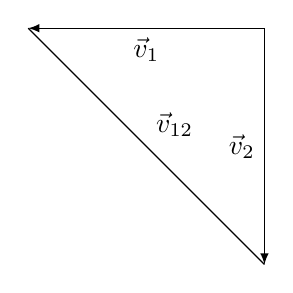
\begin{tikzpicture}[scale=2]
			\coordinate (A) at (0,0);
			\coordinate (B) at (-1.5,0);
			\coordinate (C) at (0, -1.5);
			\draw[-latex] (A) -- node[below] {$\vec{v}_1$} (B);
			\draw[-latex] (A) -- node[left] {$\vec{v}_2$} (C);
			\draw (B) -- node[above right] {$\vec{v}_{12}$} (C);
		\end{tikzpicture}
	\end{center}
	Além disso, pelo desenho,
	$$
		\sin{\theta} = \frac{|\vec{v}_{2}|}{|\vec{v}_{21}|},\quad \cos{\theta} = \frac{|\vec{v}_{1}|}{|\vec{v}_{21}|} = \frac{|\vec{v}_{2}|}{|\vec{v}_{21}|} = \sin{\theta}.
	$$
	A igualdade entre seno e cosseno ocorre quando o ângulo vale 45 graus, ou seja, $\theta = 45\deg.$ Assim,
	$$
		\vec{v}_{21} = \vec{v}_{2} - \vec{v}_{1} = -|\vec{v}_{2}|\hat{i} - (-|\vec{v}_{1}|\hat{j}) \Rightarrow \vec{v}_{21} = -|\vec{v}_{2}|\hat{i} + |\vec{v}_{1}|\hat{j}.
	$$
	Logo,
	$$
		|\vec{v}_{21}| = \sqrt{|\vec{v}_{1}|^{2} + |\vec{v}_{2}|^{2}}\approx 85km/h
	$$

	Para resolver, agora, o item b, a comecemos pela posição relativa 2 nos instantes t=0, t=2min e t=4min. Quanto ao trem 2, as
	informações que temos indicam que ele se move no eixo x ($y_{2}(t) = 0$), em t=2min, ele está na origem ($x_{2}(2min) = 0$) e, deste modo,
	$$
		\vec{r}_{2}(t) = x_{2}(t)\hat{i} + y_{2}(t)\hat{j} = x_{2}(t)\hat{i} \Rightarrow x_{2}(t) = x_{2O} + |\vec{v}_{2}|t
	$$
	Utilizando o valor que sabemos, i.e., x(2min), segue que, convertendo 2 minutos para horas ($2min\approx 0.03h$) ,
	$$
		x(0.03) = 0 = x_{2O} - 60 \cdot 0.03 \Rightarrow x_{2O} = 60 \cdot 0.03 = 2km.
	$$

	Agora, sobre o trem 1, sabe-se que ele se move no eixo y, ou seja, $x_{1}(t) - 0$, tal que
	$$
		y_{1}(t) = -|\vec{v}_{1}|t = -60t
	$$

	Com essas informaç\~es, encontramos os valores
	\begin{align*}
		 & t = 0min:\quad x_{1}(0) = 0, y_{1}(0) = 0,\quad x_{2}(0) = 2km, y_{2}(0) = 0km    \\
		 & t = 2min:\quad x_{1}(2) = 0, y_{1}(2) = -2km,\quad x_{2}(2) = 0km, y_{2}(2) = 0km \\
		 & t = 4min:\quad x_{1}(4) = 0, y_{1}(4) = -4km,\quad x_{2}(4) = -2, y_{2}(4) = 0km.
	\end{align*}
	Desta forma,
	$$
		\vec{r}_{21}(t) = \vec{r}_{2}(t) - \vec{r}_{1}(t) \Rightarrow \vec{r}_{21}(t) = x_{2}(t)\hat{i} - y_{1}(t)\hat{j}.
	$$

	Finalmente, para o item c, calculamos a disência como
	$$
		L_{21}(t) = \sqrt{x_{1}^{2} + (-y_{1})^{2}} = \sqrt{(x_{20}-|\vec{v}_{2}(t)|)^{2} + (|\vec{v}_{1}|)^{2}} = \sqrt{7200t^{2} - 240t + 4}.
	$$
	Para encontrar a distância \textbf{mínima}, é preciso derivar esta fórmula, igualar a 0 e resolver para tempo. Coloque $l = 7200t^{2}-240t+4$,
	tal que
	$$
		\frac{dl}{dt} = 2 \cdot 7200t - 240 + 0 = 0
	$$
	Resolvendo isso, encontramos o tempo em que a distância é mínima, valendo $t^{*}\approx 0.017h\approx 1min$, tal que a distância mínima é
	$$
		L_{21}(t^{*})\approx 1.4.
	$$
\end{example}
\end{document}
